This chapter covers the implementation of the text-aware process prediction model presented in the previous chapter.
In the first section the underlying technology is depicted, whereas in the second section the architecture of the implementation is described.

\section{Technology}

The implementation of the text-aware process prediction model is purely based on Python 3.6 \cite{python}.
The set of Python packages that are utilized for the implementation are summarized in Table \ref{tab:packages}.
All packages follow the open-source development model.

\begin{table}[!htbp]
	\begin{tabularx}{\textwidth}{l p{4.5cm} p{6.6cm} }
		\toprule
		\textbf{Package} & \textbf{Developer(s)} & \textbf{Purpose}  \\
		\midrule
		PM4Py \cite{DBLP:journals/corr/abs-1905-06169}   &  Fraunhofer Institute for Applied Information Technology &  Event log parsing and handling\\
		TensorFlow \cite{DBLP:journals/corr/AbadiABBCCCDDDG16} &  Google Brain Team et al.& Construction and training of LSTM model \\
		NTLK \cite{DBLP:books/daglib/0022921} & Bird et al. & Text preprocessing\\
		Scikit-learn \cite{DBLP:journals/jmlr/PedregosaVGMTGBPWDVPCBPD11} & Cournapeau et al.& Bag of words and bag of n-gram tf-idf encoding \\
		Gensim \cite{rehurek_lrec} & Řehůřek et al. & Latent Dirichlet Allocation and Paragraph Vector encoding \\
		 \bottomrule
	\end{tabularx}
	\caption[List of Python packages used for implementation]{List of Python packages used for implementation.}
	\label{tab:packages}
\end{table}

PM4Py \cite{DBLP:journals/corr/abs-1905-06169} is a python Package developed by the Fraunhofer Institute for Applied Information Technology, which offers a wide range of process mining algorithms and event log operations for the Python environment.
It is used for event log parsing and its internal event log model.

TensorFlow \cite{DBLP:journals/corr/AbadiABBCCCDDDG16} is a dataflow oriented framework originally developed by Google, which includes a huge set of neural network models and serves with its LSTM implementation using its Keras API.

Furthermore, the packages NTLK \cite{DBLP:books/daglib/0022921}, Scikit-learn \cite{DBLP:journals/jmlr/PedregosaVGMTGBPWDVPCBPD11} and Gensim \cite{rehurek_lrec} are applied for the preprocessing and encoding of textual data.
NTLK is used to realize the tokenization and word lemmatization, whereas the implementation of the text models is supported by the Scikit-learn (bag of words, bag of n-gram) and Gensim LDA, Paragraph Vector) packages.


\section{Model Implementation}

The interface of the text-aware process prediction model is realized through a class \texttt{TappModel}, which implements the functions \texttt{fit()},  \texttt{predict()} and  \texttt{evaluate()}, that can be used to fit the model to an event log with historical data, 

\begin{figure}[htbp!]
	\centering
	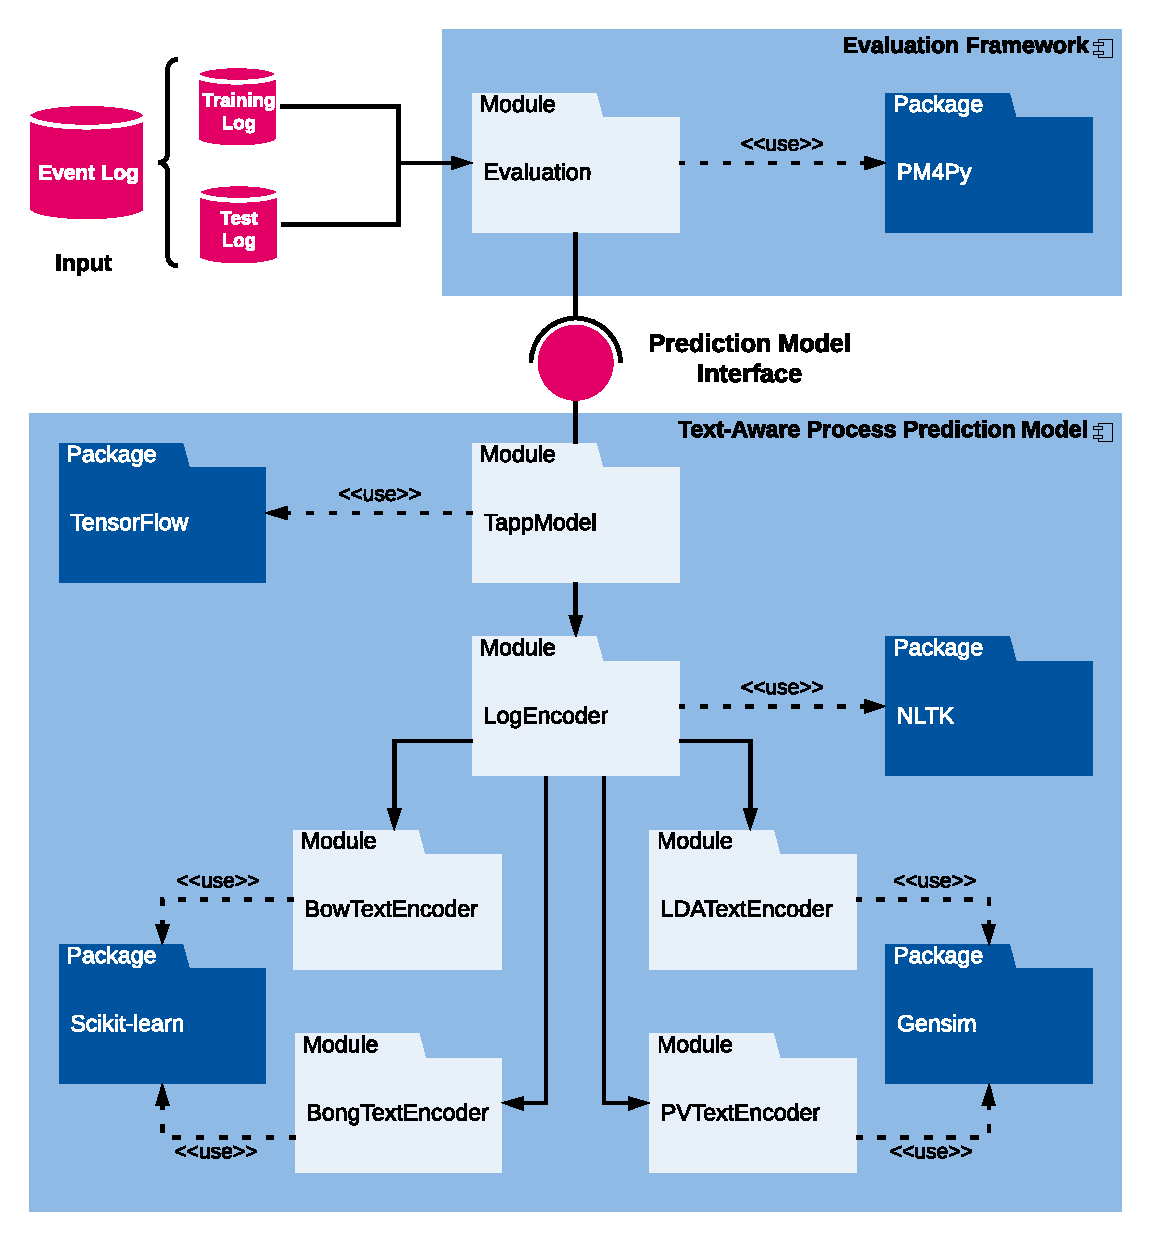
\includegraphics[width=\textwidth]{figures/implementation}
	\caption[Composition of the prediction model]{Modules and packages for the composition of the prediction model component.}
	\label{fig:/implementation}
\end{figure}